\documentclass[11pt,letterpaper,boxed]{hmcpset}
\usepackage{fullpage}
\setlength{\parskip}{6pt}
\setlength{\parindent}{0pt}
\usepackage[margin=1in]{geometry}
\usepackage{graphicx}
\usepackage{enumerate}
\usepackage{marvosym}
\usepackage{amssymb}
\usepackage{wasysym}
\usepackage{gensymb}
\usepackage{mathrsfs}
\usepackage{scrextend}
\usepackage{mathtools}
\usepackage{pgfplots}
\usepackage{xspace}
\usepackage[colorlinks]{hyperref}

\makeatletter
\renewcommand*\env@matrix[1][*\c@MaxMatrixCols c]{%
   \hskip -\arraycolsep
   \let\@ifnextchar\new@ifnextchar
   \array{#1}}
\makeatother

% --- style --- %
\renewcommand{\labelenumi}{{ (\alph{enumi})}}
\newcommand{\sand}{\quad \mbox{ and } \quad}
%\newcommand{\ds}{\displaystyle}
\allowdisplaybreaks

% --- making \xi look less awful --- %
\DeclareSymbolFont{CMletters}{OML}{cmm}{m}{it}
\DeclareMathSymbol{\xi}{\mathord}{CMletters}{"18}

% --- math --- %
\newcommand{\Z}{\mathbb{Z}}
\newcommand{\R}{\mathbb{R}}
\newcommand{\C}{\mathbb{C}}
\newcommand{\Q}{\mathbb{Q}}


\newcommand{\Lt}[1]{\mathcal{L}\crb{#1}}
\newcommand{\ilt}[1]{\mathcal{L}^{-1}\crb{#1}}

\newcommand{\pn}[1]{\left( #1 \right)}
\newcommand{\sqb}[1]{\left[ #1 \right]}
\newcommand{\crb}[1]{\left\{ #1 \right\}}
\newcommand{\lra}[1]{\left\langle #1 \right\rangle}
\newcommand{\magn}[1]{\left\lVert #1 \right\rVert}

\newcommand{\pdr}[2]{\frac{\partial #1}{\partial #2}}
\newcommand{\im}[1]{\text{im}\pn{#1}}
\newcommand{\m}[1]{\Z/#1\Z}

\newcommand{\VEC}[1]{\ensuremath{\mathbf{#1}}\xspace}
\DeclareMathOperator{\proj}{proj}
\newcommand{\vectorproj}[2][]{\proj_{\VEC{#1}}\VEC{#2}}

\newenvironment{amatrix}[1]{%
  \left(\begin{array}{@{}*{#1}{c}|c@{}}
}{%
  \end{array}\right)
}

\makeatletter
\renewcommand*\env@matrix[1][*\c@MaxMatrixCols c]{%
  \hskip -\arraycolsep
  \let\@ifnextchar\new@ifnextchar
  \array{#1}}
\makeatother

\newcommand{\spn}[1]{\text{span}\pn{#1}}

\newcommand*\Heq{\ensuremath{\overset{\kern2pt H}{=}}}

\name{Box \#$\rule{1cm}{0.15mm}$}
\class{Math 60 Section 1}
\assignment{Homework 10}
\duedate{29 May 2018}

\begin{document}

%\begin{center}
\noindent\textbf{Collaborators:} 
%\end{center} 

%\problemlist{}

\begin{problem}[Colley 6.1 \#2]
Calculate $\int_{\mathbf{x}} f\,ds$ where
\[
	f(x,y,z) = xyz, \qquad \mathbf{x}(t) = (t,2t,3t), \quad 0\leq t\leq2.
\]
\end{problem}

\begin{solution}
\vfill
\end{solution}
\newpage

\begin{problem}[Colley 6.1 \#9]
Find $\int_{\mathbf{x}}\mathbf{F}\cdot d\mathbf{s}$ where
\[
	\mathbf{F} = (y+2)\mathbf{i}+x\mathbf{j}, \qquad \mathbf{x}(t) = (\sin{t},-\cos{t}), \quad 0\leq t\leq\pi/2.
\]
\end{problem}

\begin{solution}
\vfill

\end{solution}
\newpage

\begin{problem}[Colley 6.1 \#21]
Let $\mathbf{F} = (x^2+y)\mathbf{i}+(y-x)\mathbf{j}$ and consider the two paths
\begin{align*}
	\mathbf{x}(t) &= (t,t^2), \quad 0\leq t \leq 1\\
	\mathbf{y}(t) &= (1-2t, 4t^2-4t+1), \quad 0\leq t\leq \frac{1}{2}
\end{align*}
\begin{enumerate}
\item Calculate $\int_{\mathbf{x}}\mathbf{F}\cdot d\mathbf{s}$ and $\int_{\mathbf{y}}\mathbf{F}\cdot d\mathbf{s}$.
\item By considering the image curves of the paths $\mathbf{x}$ and $\mathbf{y}$, discuss your answers in part (a).
\end{enumerate}
\end{problem}

\begin{solution}
\vfill
\end{solution}
\newpage

\begin{problem}[Colley 6.1 \#31]
Evaluate
\[
	\int_Cyz\,dx -xz\,dy+xy\,dz,
\]
where $C$ is the line segment from $(1,1,2)$ to $(5,3,1)$.
\end{problem}

\begin{solution}
\vfill
\end{solution}
\newpage

\begin{problem}[Colley 6.1 \#34]
Tom Sawyer is whitewashing a picket fence. The bases of the fenceposts are arranged 
in the $xy$-plane as the quarter circle $x^2+y^2 =25,x,y\geq0$, and the height of the fencepost at point $(x,y)$ is given by $h(x,y)=10-x-y$ (units are feet). Use a scalar line integral 
to find the area of one side of the fence.
\begin{center}
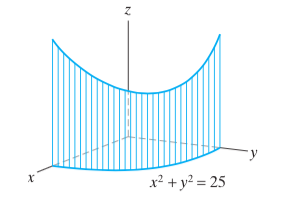
\includegraphics[scale=0.6]{sawyer.png}
\end{center}
\end{problem}

\begin{solution}
\vfill
\end{solution}
\newpage

\begin{problem}[Colley 6.1 \#40]
You are traveling through Cleveland, famous for its lake-effect snow in winter that makes driving quite treacherous. 
Suppose that you are currently located 20 miles due east of Cleveland and are attempting to drive to a 
point 20 miles due west of Cleveland. Further suppose that if you are $s$ miles from the center of Cleveland,
 where the weather is the worst, you can drive at a rate of at most $v(s) = 2s +20$ miles per hour.
 \begin{enumerate}
 \item How long will the trip take if you drive on a straight-line path directly through Cleveland? (Assume that you always drive at the maximum speed possible.)
 \item How long will the trip take if you avoid the middle of the city by driving along a semicircular path with Cleveland at the center? (Again, assume that you drive at the maximum speed possible.)
 \item Repeat parts (a) and (b), this time using $v(s) =
(s^2/16) + 25$ miles per hour as the maximum speed that you can drive.
 \end{enumerate}
\end{problem}

\begin{solution}
\vfill
\end{solution}
\newpage

\begin{problem}[Colley 6.2 \#4]
Verify Green's Theorem for the given vector field
\[
	\VEC{F}  = M(x,y)\VEC{i} + N(x,y)\VEC{j}
\]
and region $D$ by calculating both 
\[
	\oint_{\partial D} M\,dx+N\,dy \sand \int\int_D (N_x-M_y)\,dA.
\]
where 
\[
	\VEC{F} =2y\VEC{i}+x\VEC{j},
\]
and $D$ is the semicircular region $x^2+y^2\leq a^2$, $y\geq 0$.
\end{problem}

\begin{solution}
\vfill
\end{solution}
\newpage


\end{document}